\documentclass{article}
\usepackage{float}
\usepackage{graphicx}
\usepackage{amsmath}
\usepackage{listings}
\usepackage{color}
\definecolor{cadmiumgreen}{rgb}{0.0, 0.42, 0.24}
\lstset{frame=tb,
  language=R,
  aboveskip=3mm,
  belowskip=3mm,
  showstringspaces=false,
  columns=flexible,
  basicstyle={\small\ttfamily},
  numbers=none,
  numberstyle=\tiny\color{gray},
  keywordstyle=\color{blue},
  commentstyle=\color{dkgreen},
  stringstyle=\color{cadmiumgreen},
  breaklines=true,
  breakatwhitespace=true,
  tabsize=3
}
\usepackage[margin=0.75in]{geometry}
\setlength\parindent{0pt}

\title{QSCI 381 HW 3}
\date{1/20/2023}
\author{Simon-Hans Edasi}

\begin{document}

	\maketitle



%%%%%%%%%%%%%%%%%%%%%%%%%%%%%%%%%%%%%%%%%%%%%%%%%%
\section{Part 1 (questions 1-5)}








In part 1 of today’s lab, we will be using data on the number of screen devices (i.e., TVs, computers, smartphones, tablets, etc.) from a random sample of 32 households in the United States. Copy the data below into R/RStudio to create an object named “screen” using the c() function:

\begin{center}
\begin{lstlisting}
screen <- c(8, 4, 7, 7, 9, 5, 5, 6, 6, 4, 7, 9, 4, 9, 6, 7, 10, 10, 3, 4, 5, 7, 1, 9, 7, 9, 8, 13, 5, 11, 8, 3)
\end{lstlisting}
\end{center}
(1) Create a histogram with the above data. Select a color of your choice, add appropriate x and y axis labels, and add a title using commands you learned in Lab 1. Paste in your histogram below. (11 points)
\begin{center}
\begin{lstlisting}
hist(screen, main = 'Number of Screens per US Household', xlab = 'Number of Screens', ylab = 'Number of Households', col = 'orange')
\end{lstlisting}
\begin{figure}[H]
    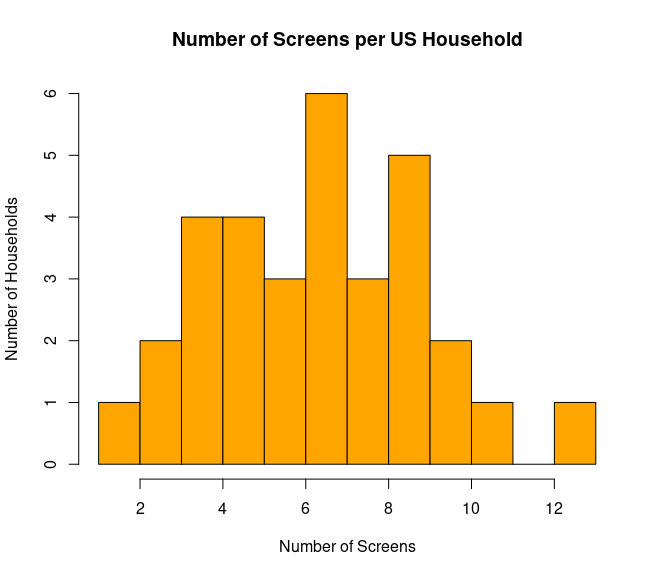
\includegraphics[scale = 0.75]{screens_histogram.png}
\end{figure}
\end{center}


(2) Based on a visual inspection of your histogram, how many screen devices would you expect the average U.S. household to have? Justify your answer. (5 points) \\

I would expect the average U.S. household to have 7 screens. Most households in the data have seven screens, and the data appears more or less normally distributed. \\

(3) Create a frequency table of the screen data using the table () command in R/RStudio. Paste your frequency table below. (5 points) \\

\begin{center}
\begin{lstlisting}
table(screen)
screen
 1  3  4  5  6  7  8  9 10 11 13 
 1  2  4  4  3  6  3  5  2  1  1 
\end{lstlisting}
\end{center}
(4) Use your frequency table from (3) to calculate the probability, Px, for each category of the number of screen devices per U.S. household. Input your individual probabilities below. Round your probabilities to three decimal places. Note: this is something you can set up in Microsoft excel (8 points)\\

\begin{center}
\begin{lstlisting}
> P_1 <- (1/sample_space) = 0.031
> P_3 <- (2/sample_space) = 0.063
> P_4 <- (4/sample_space) = 0.125
> P_5 <- (4/sample_space) = 0.125
> P_6 <- (3/sample_space) = 0.094
> P_7 <- (6/sample_space) = 0.188
> P_8 <- (3/sample_space) = 0.094
> P_9 <- (5/sample_space) = 0.156
> P_10 <- (2/sample_space) = 0.063
> P_11 <- (1/sample_space) = 0.031
> P_13 <- (1/sample_space) = 0.031
> P_san_check <- sum(P_1, P_3, P_4, P_5, P_6, P_7, P_8, P_9, P_10, P_11, P_13) = 1
\end{lstlisting}
\end{center}

Sample space $s$ is the total number of homes, or the length of the list ``screen''. Each entry $f$ is the number of screens $n$ in the home. The probability $P$ of having $n$ screens is 
\[
P_n = (f / s)
\]

(5) Use the information from (4) to estimate the expected value, or mean, of the number of screen devices per U.S. household from the random sample of 32 households. Consider the number of screen devices in the sample as a discrete random variable. Hint: calculate xP(x) first. Round your answer to three decimal places. Is your estimated mean consistent with your visual observation from the histogram and your answer in (2)? Justify your answer (10 points)\\

Expected value:
\[
 \mu = \Sigma x P_x
\]

\begin{center}
\begin{lstlisting}
sum(x1*P_1, x3*P_3, x4*P_4, x5*P_5, x6*P_6, x7*P_7, x8*P_8, x9*P_9, x10*P_10, x11*P_11, x13*P_13) = 3.813
\end{lstlisting}
\end{center}
 
%%%%%%%%%%%%%%%%%%%%%%%%%%%%%%%%%%%%%%%%%%%%%%%%%%
\section{Part 2 (questions 6-8)}


In part 2 of today’s lab, we will explore the use of three discrete probability distributions: geometric, binomial, and Poisson. Consider the following problems, use the appropriate probability distribution to solve. You will be introduced to commands available in R/RStudio to solve each problem (as opposed to solving them by hand using the formula). Showing your R/RStudio code could increase your probability of partial credit.\\

Geometric probability distribution. In R/RStudio, we can use the following command to calculate probabilities under the geometric distribution:
\begin{center}
\begin{lstlisting}
dgeom(x, prob)
\end{lstlisting}
\end{center}
in which "x" is the number of the trials prior to the event (i.e., the x-1 from the formula from lecture), and "prob" is the probability of the event.\\

As an example, consider the career free throw percentage of basketball player Stephen Curry, which is $90.8\%$. Using the geometric probability distribution, we can calculate that the probability that Stephen Curry makes his first free throw on the third free throw attempt in a game; in other words, he misses his first two attempts and makes his third attempt. Using R/RStudio, we can do this by inputting:\\
\begin{center}
\begin{lstlisting}
dgeom(2, 0.908)
\end{lstlisting}
\end {center}
which gives us 0.0077, and is the same answer as the formula:
\[
P(x) = pq^{\left(x-1\right)} = (0.908)*(1-0.908)^2 = 0.0077
\]
Use the dgeom() command in R/RStudio to complete the following:\\

(6) A manufacturer finds that 3 out of every 86 items produced is defective. Use this information to calculate the following. Round your answers to three decimal places.\\

(6a) The probability that the 1st defective item is the eighth item produced. (3 points)
\begin{center}
\begin{lstlisting}
Pd_8 <- dgeom(7, (3/86)) = 0.027
\end{lstlisting}
\end{center}

(6b) The probability that the first defective item is the 1st, 2nd, or 3rd item produced. (3 points)\\

\begin{center}
\begin{lstlisting}
> Pd_1 <- dgeom(0, (3/86)) = 0.035
> Pd_2 <- dgeom(1, (3/86)) = 0.034
> Pd_3 <- dgeom(2, (3/86)) = 0.032
\end{lstlisting}
\end{center}
(6c) The probability that none of the first 4 items produced are defective. (3 points)\\

In other words, the probability that the first 4 items are good. Sum probabilities for each frequency of items being defective. 1 - that probability is the probability they are all good.

\begin{center}
\begin{lstlisting}
> Pd_1 <- dgeom(0, (3/86)) = 0.035
> Pd_2 <- dgeom(1, (3/86)) = 0.034
> Pd_3 <- dgeom(2, (3/86)) = 0.032
> Pd_4 <- dgeom(3, (3/86)) = 0.031
> P4_good <- 1- sum(Pd_1, Pd_2, Pd_3, Pd_4) = 0.868

\end{lstlisting}
\end{center}


(6d) The probability that when inspecting a batch of 30 items, that the first defective item is found after the 3rd item is inspected. (3 points)\\

In other words: What is the probability the fourth item is defective out of a batch of 30? Using the failure rate of $3/86$, we can expect 1 item to be defective from a batch of 30 $(30 * (3/86))$. The chances of this 1 defect is found after the third item is inspected is:

\begin{center}
\begin{lstlisting}
P_4th_defect <- dgeom(3, (1/30)) = 0.030	
\end{lstlisting}
\end{center}

Binomial probability distribution. In R/RStudio, we can use the following command to calculate probabilities under the binomial distribution:
\begin{center}
\begin{lstlisting}
dbinom(x, size = n, prob = p)
\end{lstlisting}
\end{center}

in which "x" is the frequency of the first outcome, n is number of independent experiments or trials, and prob = p, or the probability of the first outcome occurring. Because q is 1 - p, we only need to provide R/RStudio with p, from which the software can deduce q.\\

Consider the probability of selecting exactly 2 adults who have blood type A from a random sample of 3 adults, and assume that the probability of having blood type A is 0.42. In this case, x=2, n=3, and prob=0.42. Using R/RStudio, we can solve this problem this by inputting:
\begin{center}
\begin{lstlisting}
dbinom(2, size=3, prob=0.42) = 0.3069
\end{lstlisting}
\end{center}


Use the dbinom () command in R/RStudio to complete the following:\\

(7) Among U.S. adults, 32\% say that strawberry is their favorite flavor of ice cream. You randomly select 25 adults and ask them to name their favorite flavor of ice cream. Use this information to calculate the following. Round your answers to three decimal places.\\



(7a) Find the probability that the number of adults from the random sample who say strawberry is their favorite flavor of ice cream is exactly 8. (3 points)\\

(7b) Find the probability that the number of adults from the random sample who say strawberry is their favorite flavor of ice cream is 4 or less. (3 points)\\

(7c) Find the probability that the number of adults from the random sample who say strawberry is their favorite flavor of ice cream is 5 or more. (3 points)\\

(7d) From the random sample of 25 adults, what is the mean, variance, and standard deviation of the number of adults that say strawberry is their favorite flavor of ice cream? (3 points)\\

 

Poisson probability distribution. In R/RStudio, we can use the following command to calculate probabilities under the Poisson distribution:
\begin{center}
\begin{lstlisting}
dpois(x, lambda=mean)
\end{lstlisting}
\end{center}

in which x is the number of occurrences, and lambda is the mean number of occurrences.\\

Consider the number of vacancies on the U.S. Supreme Court in which the mean number of vacancies is 0.484 per year. We can use R/RStudio to calculate the probability of having 0 or 1 vacancies in a year by inputting:
\begin{center}
\begin{lstlisting}
dpois(0, lambda=0.484) + dpois(1, lambda=0.484) = 0.915
\end{lstlisting}
\end{center}

Use the dpois() command in R/RStudio to complete the following:\\

(8) Occasionally an airline will lose a checked bag. An airline company has determined that it can estimate the number of checked bags lost each weekday using the Poisson distribution with a mean of 2.6 checked bags lost per weekday. Use this information to calculate the following. Round your answers to three decimal places.\\


(8a) What is probability that the airline company will lose no checked bags next Monday? (3 points)
\begin{center}
\begin{lstlisting}
dpois(0, lambda = 2.86) = 0.057
\end{lstlisting}
\end{center}

(8b) What is probability that the airline company will lose 3 or fewer checked bags next Monday? (3 points)\\
\begin{center}
\begin{lstlisting}
dpois(0, 2.86) + dpois(2, 2.86) + dpois(2, 2.86) + dpois(3, 2.86) = 0.749
\end{lstlisting}
\end{center}
(8c) What is probability that the airline company will lose 2 or more checked bags next Monday? (3 points)
\begin{center}
\begin{lstlisting}
dpois(0, 2.86) + dpois(1, 2.86) + dpois(2, 2.86) = 0.679
\end{lstlisting}
\end{center}
(8d) What would be an unusually high number of checked bags lost by the airline company on a given weekday? Justify your answer. (3 points)\\
\begin{center}
\begin{lstlisting}
dpois(2,2.86) = 0.2342178
dpois(3,2.86) = 0.2232876
dpois(4,2.86) = 0.1596506
dpois(5,2.86) = 0.09132017
dpois(6,2.86) = 0.04352928
\end{lstlisting}
\end{center}
Based on these results, I think 5 bags is an unusually large number because the difference in probability from 4 to 5 bags is the largest difference of probabilities. This leads me to think of a sharp dropoff between 4 and 5 bags, making 5 an unusual occurence.
\end{document}
